\chapter{Using light waves to measure small distance changes (Michelson interferometer)}

% todo switch to pressure switches instead of toggles on lasers - more stationary

With the basic properties of waves and wave interference established (via the ripple tank) and the same behavior
demonstrated in light (via the laser-based modern version of Young's double slit experiment) we are now finally ready to
look at a Michelson interferometer. This technology is the basis of the LIGO experiment. You may want to refer back to
the introduction of Lab~\ref{cha:ripple-tank} to remind yourself of some details. LIGO itself is a large experiment that has
been constructed over several decades of work and technology development, and so is many orders of magnitude more
precise and sensitive than what we can do in an hour on a lab bench. Nevertheless, the basic principles are the same.

Figure~\ref{mi:fig:schematic} shows a diagram of a Michelson interferometer. A beam of light from the laser source of wavelength $\lambda$
strikes the beam-splitter. The beam-splitter $B$ is designed to reflect 50\% of the incident light and transmit the other 50\%.
The incident beam therefore splits into two beams; one beam is reflected toward mirror M$_1$, the other is transmitted
toward mirror M$_2$. M$_1$ and M$_2$ reflect the beams back toward the beam-splitter. Half the light from M$_1$ is transmitted
through the beam-splitter to the viewing screen and half the light from M$_2$ is reflected by the beam-splitter to the
viewing screen.

\begin{figure}
	\centering
	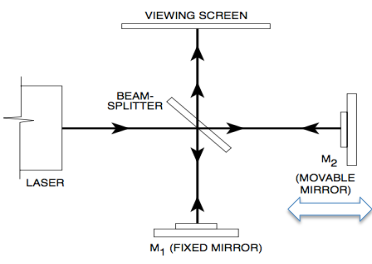
\includegraphics[width=0.5\textwidth]{michelson-interferometer/michelson-schematic.png}
	\caption{Schematic of a Michelson interferometer.}\label{mi:fig:schematic}
\end{figure}

In this way the original beam of light splits, and portions of the resulting beams are brought back together. The
beams are from the same source and their phases are hence highly correlated. When mirror $M_2$ is moved (closer to or
further from the laser source) the \textit{difference} in the path length of the light beams $(B$M$_1 - B$M$_2)$ changes, resulting in
changed in interference fringes. For a clear visualization of the effect, a lens placed between the laser source and the
beam-splitter spreads out the beam. An interference pattern of dark and bright rings, or \textit{fringes}, is seen on the
viewing screen. The rings are generated by interference of different portions of the laser beam, expanded to easy
visibility by the lens.

\section{Setup and Alignment of the interferometer}

Before you do an experiment with the interferometer, you'll need to ensure that it is aligned and an interference pattern (a set of concentric alternating light and dark rings) is clearly seen on the viewing screen when the laser is turned on. If that's true, then you can skip ahead to the next section.

Our laboratory setup is shown in Figure~\ref{mi:fig:setup-photo}.

\begin{framed}
	\textbf{Warning: Laser Hazard!} Lasers can cause temporary and permanent damage to eyes when exposed directly or through reflective surfaces.
	
	The following rules reduce the risk of eye exposure to laser light:
	\begin{enumerate}
		\item Do not direct the laser beam into anyone's eye.
		\item Be aware of the laser reflecting off of mirror-like surfaces and where that beam goes.
		\item Turn off the laser when not in use.
		\item Keep the laser pointing horizontally and near the plane of the table, while keep your eyes above that plane.
		\item To determine whether the laser is on, put your hand or a light-colored object in front of the beam, rather than looking into the laser aperture.
	\end{enumerate}
\end{framed}

\begin{figure}
	\centering
	\includegraphics[width=\textwidth]{michelson-interferometer/setup-photo.png}
	\caption{Our particular classroom setup, fully assembled and aligned, showing an interference pattern on the viewing screen.}\label{mi:fig:setup-photo}
\end{figure}

\begin{enumerate}
	\item The interferometer itself (this is part that has the optics) should be bolted to an optical rail at one end, with the
beamsplitter mirror facing the long end of the rail. Do so, if this isn't already in place.

	\item An aluminum block, with upward
facing magnets, should also be bolted into the rail near the other end.

	\item A steel plate, with an upturned edge, should
also be bolted to the rail, with the flat edge tight against edge of the interferometer.

	\item A 3⁄4” thick steel block, with two V-shaped grooves (one large and one small) should be placed on top of the aluminum block with magnets, with the V-shaped grooves facing upward; the magnets will keep the steel block in place.
	
	\item To begin, orient the block so the V-shaped grooves are aligned with the long axis of the rail, and the larger groove is toward the side of the rail opposite from the position of M$_1$ in the interferometer. The grooves are mount points for lasers, of two different barrel widths.
	
	\item Place a laser in one of the V-shaped grooves, pointed toward the interferometer, and turn it on. If necessary, you may secure the laser to the block using an elastic band or similar, taking advantage of the small grooves on the underside of the block that allow easy passage of a securing band.
	
	\item Place a viewing screen so that it is opposite M$_1$, or use a convenient light-colored wall.
	
	\item Loosen the thumbscrew that holds the beam-splitter and rotate the beam-splitter so it is out of the beam path of the
	laser as shown in Figure~\ref{mi:fig:adjusting-m1}.
	
	\begin{figure}
		\centering
		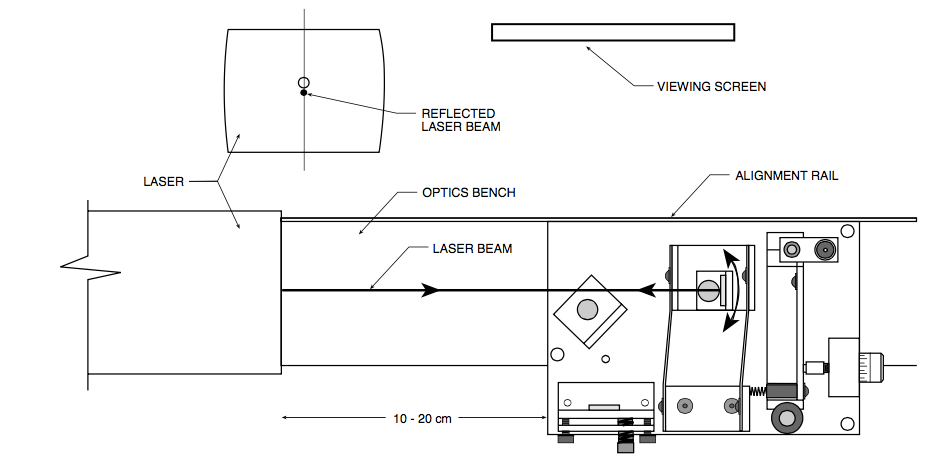
\includegraphics[width=\textwidth]{michelson-interferometer/adjusting-m1.png}
		\caption{Adjusting the M$_1$ mirror.}\label{mi:fig:adjusting-m1}
	\end{figure}
	
	\item Align the steel block holding the laser so that the beam hits M$_2$ as well-centered as
	possible; you can slide the steel block, rotate it (the magnets hold it in place but allow freedom of movement), and place paper in the groove under the laser to adjust the height or angle.
	Your goal should be to have the laser beam parallel to the long axis of the optical rail, and centered on M$_2$.
	
	\item The reflected beam should return back to the laser head. (The reflected beam need not be --- and likely won’t be --- at the
	same height as the incident beam, but it should return along the same path when viewed from exactly above. Hold
	your hand or piece of paper near the laser head --- without blocking the outgoing beam --- to see where the return beam
	is going.) If the return beam is not going where you want, you may loosen the thumbscrew that holds M$_2$ and adjust
	the rotation of M$_2$ so the laser beam is reflected directly back toward the laser head. Once satisfied with the alignment,
	hold M$_2$ in position and tighten the thumbscrew.
	
	\item Adjust the alignment screws on the mount for the mirror M$_2$, so that the mount plate does not appear tilted (see Figure~\ref{mi:fig:aligning-spots} for the location of these screws). When viewed from above there is gap between the plate holding the mirror and a
	second plate behind it. Adjust the screws so the plates appear parallel.
	
	\begin{figure}
		\centering
		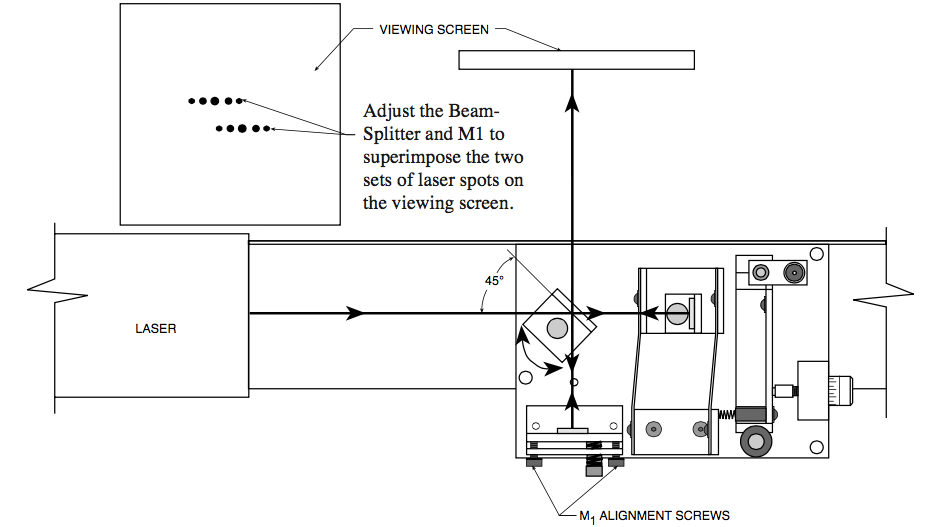
\includegraphics[width=\textwidth]{michelson-interferometer/aligning-laser-spots.png}
		\caption{Aligning the laser spots.}\label{mi:fig:aligning-spots}
	\end{figure}

	\item Rotate the beam-splitter so its surface is at an angle approximately 45 with the incident beam from the laser (see Figure~\ref{mi:fig:aligning-spots}). You will see two sets of laser spots on the viewing screen, corresponding to the two paths that the beam takes in reaching the screen. (Each path results in more than one laser spot because of multiple reflections within the beam-
	splitter.) Adjust the beam-splitter so the two sets of laser spots are as close as possible, then tighten the thumbscrew
	to secure the beam-splitter.
	
	\item Now, using the alignment screws, adjust the angle of M$_1$ until the two sets of laser spots are superimposed on the
	viewing screen (the two brightest spots must be superimposed).
	
	\item Place the 18 mm focal length lens on the optical bench on the steel plate between the laser mount and the
	interferometer (see Figure~\ref{mi:fig:positioning-lens} for setup and resulting desired pattern). The lens is in a holder that is magnetically coupled to a base; align one long edge of the base along the
	upturned edge of the steel plate. The lens should be about 10cm from the beamsplitter. Adjust the position of the lens
	on the holder so the light from the laser, now spread out by the lens, strikes the center of the beam-splitter. Move the
	lens vertically by sliding the lens holder vertically against the base (the magnets again allow freedom of movement
	here. The simplest way to move lens horizontally is to just slide the base lone the edge of the steel plate below. You
	should see an illuminated oval (or at least a partially illuminated oval) of laser light on the viewing screen. Adjust the
	lens position until the oval is as uniformly illuminated as you can achieve. Now, if you have performed the alignment
	correctly, you will see not just an illuminated oval, but a interference pattern of concentric rings on the viewing screen.
	If the alignment is not just right, the center of the fringe pattern may not be visible on the screen. Adjust the alignment
	screws on M$_1$ very slowly as needed to center the pattern. \textit{NOTE: aligning the interferometer so that you get fringes
	can be fiddly...if necessary, try a few times, and seek help from your TA if you cannot make it work.}

	\begin{figure}
		\centering
		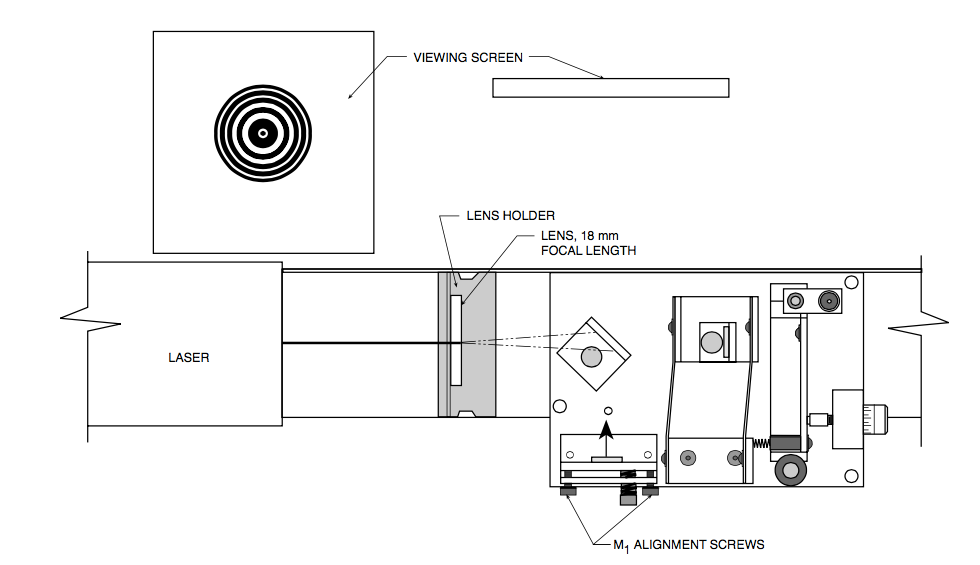
\includegraphics[width=\textwidth]{michelson-interferometer/positioning-lens.png}
		\caption{Positioning the lens, and fine alignment of M$_1$.}\label{mi:fig:positioning-lens}
	\end{figure}

\end{enumerate}

\section{Relating wavelength to distance changes}

By moving the mirror M$_2$, the path length of one of the beams can be varied. Since the beam traverses the path
between M$_2$ and the beam-splitter twice, moving M$_2$ 1/4 wavelength nearer to the beam-splitter will reduce the optical
path of that beam by 1/2 wavelength. The interference pattern will change; the radii of the maxima will be reduced so
they now occupy the position of the former minima. If M$_2$ is moved an additional 1/4 wavelength closer to the beam-splitter, the radii of the maxima will again be reduced so maxima and minima trade positions. However, this new
arrangement will be indistinguishable from the original pattern. So when moving the position of M$_2$, you will observe the
fringes ``moving'' reproducing the original pattern.

The movement distance $d$ of the mirror M$_2$ and the corresponding number of times $m$ the fringe pattern is restored to its original state are related by
\begin{equation}\label{mi:eq:interference}
 m \lambda = 2 d \, ,
\end{equation}
where $\lambda$ is the wavelength of the incident light. Thus, very small displacements d can be measured by counting the number m. Conversely, the wavelength of the light
can be accurately determined if d is known. In your interferometer, a knob with a micrometer scale can be used to move
M$_2$. M$_2$ is help on a lever spring arm that is anchored to the baseplate of the interferometer at another location. The
micrometer knob pushes on another arm that applies tension to a strap that is coupled to the lever arm holding M$_2$.

\section{Experiment 1: determining the wavelength of the laser}

\textbf{Goal:} Determine the wavelength of a laser.

\textbf{Rubric rows to be assessed:} D1, D4, F1, F2, G2, G4, G5.

\textbf{Available equipment:} Michelson interferometer mounted on optical rail, laser

Since this is such a sensitive measurement, we provide a measurement procedure for you. In order to determine the wavelength, you'll measure the number of fringes moved and the distance the mirror moved  and use Equation~\ref{mi:eq:interference} to calculate the wavelength of the laser.

\subsection{Procedure}

\begin{enumerate}
	\item\label{mi:step:micro} Adjust the micrometer knob so the lever arm is approximately parallel with the short edge of the interferometer
	baseplate. In this position the relationship between knob rotation and mirror movement is most nearly linear.
	
	\item Turn the micrometer knob one full turn counterclockwise. Continue turning counterclockwise until the zero on the
	knob is aligned with the index mark. \textit{(NOTE: Whenever you reverse the direction in which you turn the micrometer
	knob, there is a small amount of give before the mirror begins to move. This is called mechanical backlash, and is
	present in any mechanical system involving reversals in direction of movement. By beginning with a full
	counterclockwise turn, and then turning only counterclockwise when counting fringes, you can eliminate backlash
	in your measurement.)}

	\item Place a sheet of paper on the viewing screen, secure it with tape, and make a reference mark on the paper between
	two of the fringes. This will help you in keeping count of the fringes.
	
	\item Now turn counterclockwise the knob until you have counted about 40 movements of the fringes.
	
	\item\label{mi:step:record} Record the measurement on the knob as distance $d$ and record the number of fringe movements $m$.
	
	\item Repeat Steps~\ref{mi:step:micro}--\ref{mi:step:record} 2 more times, for a total of 3 measurements.
\end{enumerate}

Use your findings to determine the wavelength of the laser, including an estimate of the uncertainty in your reported value. Include the following in your report:
\begin{enumerate}
	\item A statement of the problem you are solving (D1).
	
	\item A clear, concise description of the experimental setup and procedure (F1).
	
	\item A table of the data that you took (G4).
	
	\item A description of your analysis that led you to find the wavelength (G5).
	
	\item A description, with calculations shown, of your determination of the uncertainty in the wavelength (G2).
	
	\item A final judgment of what your team thinks the wavelength of the laser is, based on your experimental results, including uncertainty (D4).
	
	\item A discussion of the findings of the experiment and why it's helpful (for you and/or for science) (F2).
\end{enumerate}

\section{Experiment 2: Measuring distance changes}

In your individual homework, you will determine distance changes in one of the arms of the interferometer, not caused by gravitational waves, like in LIGO, but by thermal expansion and the slight bending of the baseplate of the apparatus. During lab, take the following data, both without turning the knob to move the mirror:

\begin{enumerate}
	\item The clear strap that pulls the mirror back and forth will expand and contract with heating and cooling (like most solids). Measure the number of fringe movements that happen when you hold your finger very close to the strap, within a few millimeters, for 20--30 seconds.
	
	\item The baseplate is very sturdy, yet still bends when uneven pressure is applied, even if imperceptible to our senses. Measure the number of fringe movements that happen when you press lightly on the baseplate between one of the mirrors and the beam-splitter.
\end{enumerate}

\section{Individual homework}

\begin{enumerate}
	\item Use the data taken during Experiment 2 to determine the path length changes in each case (include calculation of uncertainty).
	
	\item Report on if this is surprising to you or not, either that the distance change is as large or small as it is, or the fact that you can measure such a small distance change.
	
	\item For what useful or fun purpose could this kind of sensitive measurement technique be used?
\end{enumerate}
